\subsection{Description}
%Describe where the energy meter is mounted and how, etc.

The energy meter is mounted in Service Box, which also contains power cable terminals and \gls{bspd}. Energy meter will have dedicated space in Service box with stoppers preventing it from moving. 

\subsection{Wiring, cables, current calculations, connectors}
%Describe the wiring, show schematics, provide calculations for currents and voltages, and show data regarding the cables and connectors used.

The energy meter is powered from \gls{ecub} (part of Harness\_G) with connector G$_1$ to Service box. Voltage measuring is done by connecting Energy meter to power cable terminals, which are also in Service box. This is done by Olflex Heat 180 SiF wires rated for 500 V and size AWG 17. Having power terminals in Service box allow us to measure current using current probe, or by connecting Energy meter directly to Tractive system path(both poles are possible). This is also done by Olflex Heat 180 SiF wires, but with cross-sectional area of 16mm2 and rated for 500 V and 165A. For power cable datasheet see \ref{app:PowerConductor}

\subsection{Position in car}
%Provide CAD-renderings showing all relevant parts. Mark the parts in the rendering, if necessary.

Energy meter is placed in box we call “Service Box”. The box is carbon fiber lined with FR-4 from inside. Position in car is shown below in \ref{fig:ServiceBox-position}.

\begin{figure}[H]
	\centering
	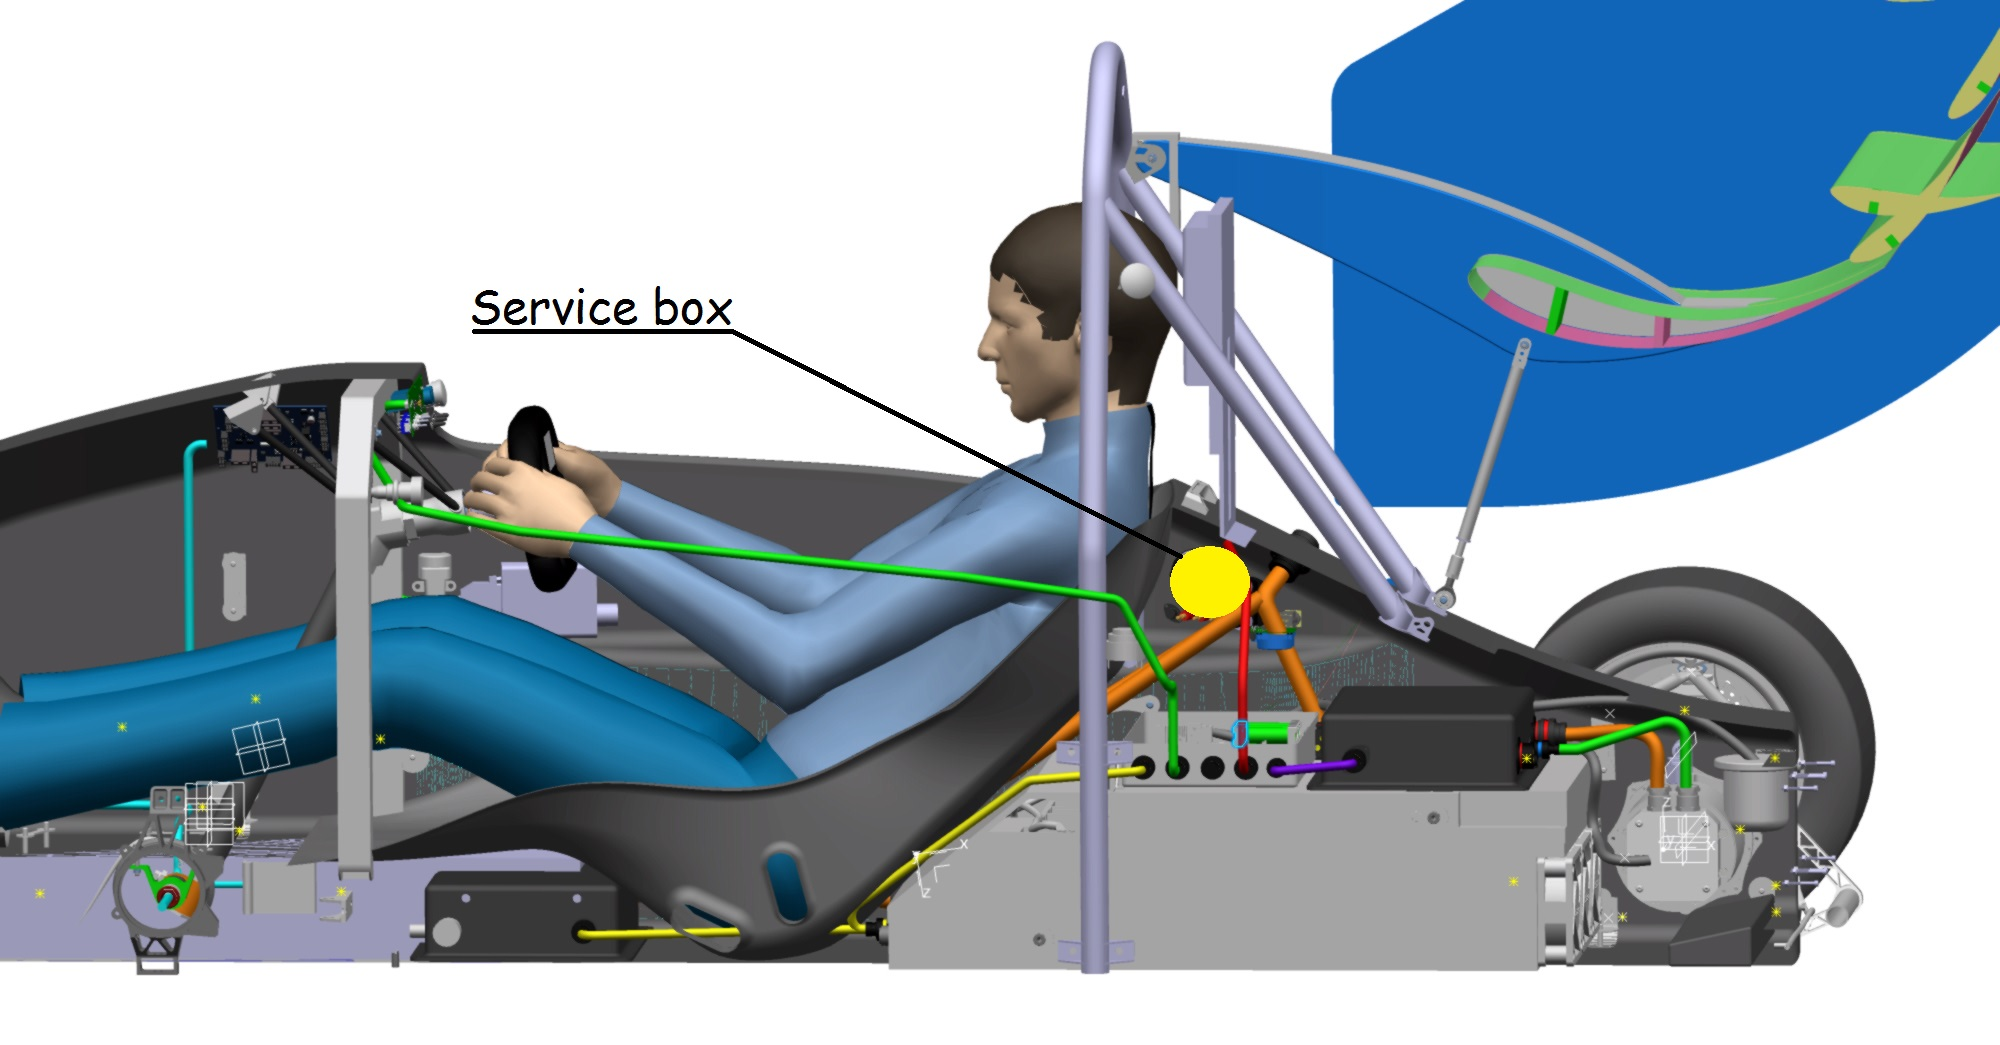
\includegraphics[width=\textwidth]{./img/ServiceBox-position.jpg}
	\caption{Service box position.}
	\label{fig:ServiceBox-position}
\end{figure}





